\section{Transfer Reward Function}

We can derive the Transfer Reward Function (TRF) as a power function with coefficients $a$ and $b$ as follows:

\begin{equation} \label{trf}
    w_m = a\cdot p_m^b = a\cdot p_m^{-1}.
\end{equation}

For $a$, we can evaluate

\begin{equation} \label{trf2}
    a = \frac{1}{M}
    \begin{dcases}
    \frac{\Xi}{ATX} & \mu \leq g \\
    g & \mu > g
    \end{dcases},
\end{equation}

where $M$ is the number of divisions, $\Xi$ is the size of the reward pool, and $ATX$ is the average annual number of transactions. We can see that $\mu = \Xi/ATX$.


A normalized graph of (\ref{trf}) can be seen below in \autoref{fig1}. 

\begin{figure}[hb]
    \centering
    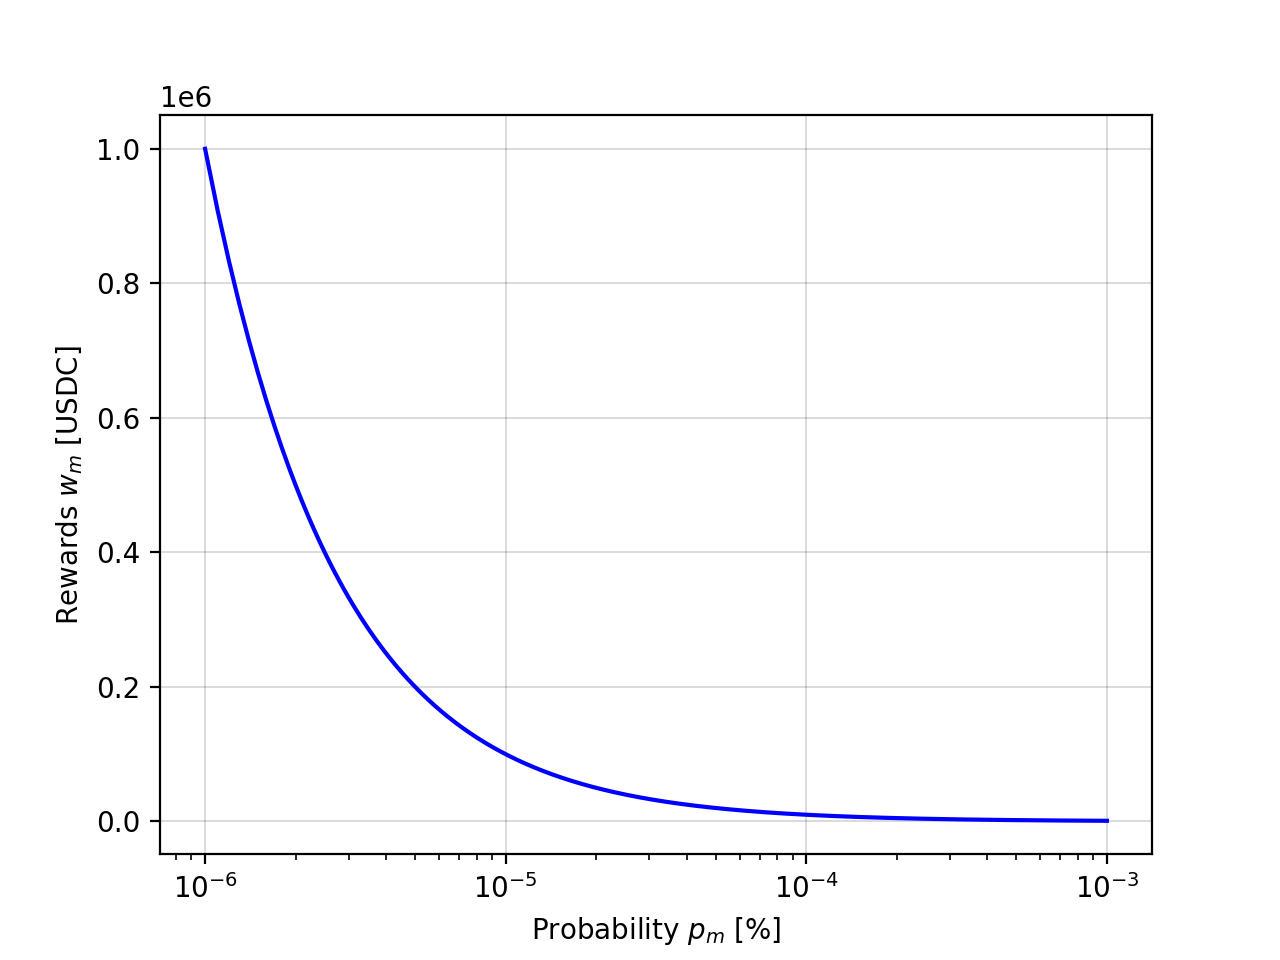
\includegraphics[width=10.5cm]{images/Figure_1.png}
    \caption{Normalized log-plot of the TRF} \label{fig1}
\end{figure}

Observing (\ref{trf2}) in detail shows that for lower volumes the reward payouts will be greater, revealing the TRFs self-regulating property due to variations in utility. As the staked pool increases over time, the rewards grow with it and the protocol will be able to "support" and attract more users.

In the following section we introduce an extension of the TRF with the Elastic Sigmoid Curve, a multiplier coefficient intended to incentivise users to engage more with the protocol by rewarding them based on their behaviour, such as staking LP tokens or locking governance tokens.